%   ####
%
%   Band VIII, 3 N.~??A11
%   Signatur/Tex-Datei: LH_35_09_15_002-005
%   RK-Nr. 41153
%   Überschrift: Motuum restitutionis regula
%   Datierung: [Dezember 1680]
%   WZ: 8-blättrige Rosette auf Zahl CS (Bl. 3-4) (RK-WZ: 138)
%   SZ: (keins)
%   Bilddateien (PDF): LH_35_09_15_002-005_d1; LH_35_09_15_002-005_d2a; LH_35_09_15_002-005_d2b; LH_35_09_15_002-005_d3; LH_35_09_15_002-005_d4; LH_35_09_15_002-005_d5; LH_35_09_15_002-005_d6; (insgesamt 7)
%
%
\begin{ledgroupsized}[r]{120mm}
\footnotesize
\pstart
\noindent\textbf{Überlieferung:}
\pend
\end{ledgroupsized}
\begin{ledgroupsized}[r]{114mm}
\footnotesize
\pstart \parindent -6mm
\makebox[6mm][l]{\textit{L}}%
Konzept: LH~XXXV~9,~15 Bl.~2\textendash5.
Zwei Bogen 4\textsuperscript{o} (Bl.~2,~5 und Bl.~3\textendash4);
ein Wasserzeichen im Falz von Bl.~3\textendash4. % Achtblättrige Rosette auf CS
Acht teilweise einspaltig beschriebene Seiten.
% Zahlreiche Streichungen, Ergänzungen und Ersetzungen.
Textfolge gemäß Blattzählung, aber nicht durch Kustoden oder weitere Hinweise von Leibniz festgelegt.
 % : Bl.~2, 5, 3 und 4.
% Auf Bl.~4~r\textsuperscript{o} Leibnizens eigenhändiger Vermerk:
% \textit{In hac pagina non est error.}
\pend
\end{ledgroupsized}
%
\vspace*{5mm}
\begin{ledgroup}
\footnotesize
\pstart
\noindent%
\textbf{Datierungsgründe:}
Der vorliegende Text N.~9 hängt inhaltlich mit den \textit{Tentaminum de chordarum tensione schedae} (N.~8) zusammen, die Leibniz auf Dezember 1680 datiert hat.
Die Über\-ein\-stim\-mung besteht insbesondere darin, dass in N.~8\textsubscript{4} und 8\textsubscript{5} der \textit{motus restitutionis} einer gespannten Saite mit\-hilfe derselben trigonometrischen Funktionen erfasst wird wie in N.~9.
Dies\-be\-züg\-lich finden sich in N.~8\textsubscript{4} (S.~\refpassage{LH_35_09_15_013r-sintheor-1}{LH_35_09_15_013r-sintheor-3}; \refpassage{LH_35_09_15_013v-sintheor-4}{LH_35_09_15_013v-sintheor-2}) auch Anspielungen, die aller Wahr\-schein\-lich\-keit nach auf N.~9 hindeuten.
Folglich muss N.~9 vorgelegen haben, als N.~8\textsubscript{4} und 8\textsubscript{5} verfasst wurden.
Das in einem Textträger von N.~9 anzutreffende Wasserzeichen, welches in den Textträgern von N.~8 ebenfalls vorkommt, ist im Leibniz-Nachlass für die frühen Hannoveraner Jahre (ab 1678) mehrfach belegt.
Der starke inhalt\-li\-che Zusammenhang % , welcher etwa auf S.~\refpassage{}{}?? und \refpassage{}{}?? besonders deutlich wird, 
ist jedoch Grund für die Vermutung, dass N.~9 etwa zur gleichen Zeit wie N.~8 entstanden ist, d.h. im Dezember 1680.
Leibniz dürfte sich \textendash\ etwas ungenau \textendash\ auf N.~9 beziehen, als er am 6. (16.) Dezember 1680 an Schelhammer schreibt, \textit{vibrationum leges ... ex intima Geometria} ergründet zu haben (\textit{LSB} III,~3 N.~139, S.~305.5\cite{01275}).
% Die Datierung von N.~??A10 wird demgemäß auch für N.~??A11 angenommen.
% Wiederum deutet N.~??A11 an einer Stelle (S.~\refpassage{}{}??) aller Wahr\-schein\-lich\-keit nach auf N.~??A10\textsubscript{??} hin.
% Diese verschränkten Verweise sind Grund zur Vermutung, dass N.~??A11 etwa zur gleichen Zeit wie N.~??A10 entstanden ist.
% Die Vermutung wird dadurch bekräftigt, dass auf Bl.~3\textendash4 das gleiche Wasserzeichen anzutreffen ist wie in den Textträgern von N.~??A10.
% Demgemäß wird die Datierung von N.~??A10 auch für N.~??A11 angenommen.
% ??? Freilich ist N.~??A11 später entstanden als die auf den Sommer 1676 zurückgehende Endfassung
% der (nie veröffentlichten) Abhandlung \cite{01229}\textit{De quadratura arithmetica circuli},
% wie eine Anspielung im Text zeigt (siehe unten,
% S.~\refpassage{LH_35_09_15_002r-tetragonismus-1}{LH_35_09_15_002r-tetragonismus-2}). ???

\pend
\end{ledgroup}
\count\Bfootins=1000
\count\Afootins=1000
\count\Cfootins=1000
%
\vspace*{4mm}
\pstart%
\normalsize%
\noindent%
%
\lbrack2~r\textsuperscript{o}\rbrack% Blatt 2r
%
\edlabel{LH_35_09_15_002r_titel-1}
\edtext{}{%
{\xxref{LH_35_09_15_002r_titel-1}{LH_35_09_15_002r_titel-2}}%
{\lemma{\lbrack2~r\textsuperscript{o}\rbrack}\Bfootnote{%
\textit{(1)}~De M
\textit{(2)}~Motuum%
~\textit{L}}}}
\pend%
% \vspace*{-0.5em}%
% Überschrift
\pstart%
\centering%
Motuum\edlabel{LH_35_09_15_002r_titel-2}
restitutionis\protect\index{Sachverzeichnis}{motus restitutionis}
regulam\protect\index{Sachverzeichnis}{regula} % \\
ita investigare conatus sum
\pend%
\vspace{0.5em}%
%
\pstart%
\noindent%
Sit
%\edtext{spatium\protect\index{Sachverzeichnis}{spatium restitutionis}
%$AB$ a quo}{%
%\lemma{spatium}\Bfootnote{%
%\textit{(1)}~in q
%\textit{(2)}~$AB$
%\textit{(a)}~in quod
%\textit{(b)}~a quo%
%~\textit{L}}}
\edtext{spatium\protect\index{Sachverzeichnis}{spatium restitutionis}
\edtext{$AB$}{%
\lemma{spatium $AB$}\Cfootnote{%
Vgl. das Diagramm \lbrack\textit{Fig.~1}\rbrack\ auf S.~\pageref{LH_35_09_15_002r_fig.1}.}}
a quo}{%
\lemma{spatium}\Bfootnote{%
\textit{(1)}~in q
\textit{(2)}~$AB$
\textit{(a)}~in quod
\textit{(b)}~a quo%
~\textit{L}}}
corpus vi diductum se restituere\protect\index{Sachverzeichnis}{corpus se restituens}
\edtext{debet
ut si chordae\protect\index{Sachverzeichnis}{chorda tensa}
$RB$ punctum $B$ adductum sit usque in $A,$
erit spatium $BA$ praeternaturale.\protect\index{Sachverzeichnis}{spatium praeternaturale}
Impetus\protect\index{Sachverzeichnis}{impetus restitutionis}}{%
\lemma{debet}\Bfootnote{%
\textit{(1)}~Impetus
\textit{(2)}~ut si chordae $RB$
\textit{(a)}~diducta
\textit{(b)}~punctum
\textit{(aa)}~$A$
\textit{(bb)}~$B$ adductum \lbrack...\rbrack\ praeternaturale. Impetus%
~\textit{L}}}
autem restitutionis sit ut $CF,$
eoque impetu $A$
\edtext{percurrere vel absolvere intelligatur}{%
\lemma{percurrere}\Bfootnote{%
\textit{(1)}~intelligatur
\textit{(2)}~vel absolvere intelligatur%
~\textit{L}}}
partem spatii infinite parvam\protect\index{Sachverzeichnis}{pars spatii infinite parva}
\edtext{$AG,$ tempore}{%
\lemma{$AG,$}\Bfootnote{%
% \hspace*{-0,5mm}
\textbar~quam vocemus $\beta$ \textit{gestr.}~%
\textbar\ tempore%
~\textit{L}}}
infinite parvo $CD,$\protect\index{Sachverzeichnis}{tempus infinite parvum}
quod vocemus $d\overline{t}.$
Secundo jam momento\protect\index{Sachverzeichnis}{momentum temporis}
seu tempusculo $DE,$\protect\index{Sachverzeichnis}{tempusculum}
quod priori ponamus aequale adeoque etiam $d\overline{t},$
impetus\protect\index{Sachverzeichnis}{impetus restitutionis}
qui imprimetur corpori restituendo\protect\index{Sachverzeichnis}{corpus restituendum}
erit minor quam ante,
quia pars restitutionis\protect\index{Sachverzeichnis}{restitutio}
praecedenti tempusculo\protect\index{Sachverzeichnis}{tempusculum} jam facta est,
et eo minor est conatus restitutionis,\protect\index{Sachverzeichnis}{conatus restitutionis}
quo minor superest tensio.\protect\index{Sachverzeichnis}{tensio}
Sunt autem
\edtext{tensiones ejusdem chordae\protect\index{Sachverzeichnis}{tensio chordae}
diductae ut spatia}{%
\lemma{tensiones}\Bfootnote{%
\textit{(1)}~ut spatium
\textit{(2)}~ejusdem chordae diductae ut spatia%
~\textit{L}}}
praeternaturalia,\protect\index{Sachverzeichnis}{spatium praeternaturale}
quod totum fuit $AB.$
Nunc restat tantum $GB.$
Ergo impetus secundus\protect\index{Sachverzeichnis}{impetus restitutionis}
$DH$ est ad priorem $CF,$
ut $BG$ est
\pend
\newpage
%\rule[0pt]{0mm}{14pt}%
%\protect\rule[-4mm]{0mm}{10mm}
  \centerline{\includegraphics[width=0.64\textwidth]{gesamttex/edit_VIII,3/images/LH_35_09_15_002-005_d1.pdf}}%\\
  \vspace{0.5em}
  \centerline{\lbrack\textit{Fig.~1}\rbrack}%
  \label{LH_35_09_15_002r_fig.1}%
%
 \vspace{1.5em}%
% \newpage%    ! ! ! ! !    REIN VORLÄUFIG    ! ! ! ! !
\pstart
\noindent ad $BA.$
Sit $AB$ aeq. $a,$
et $CF$ aequ. $b,$
et $DH$ aequ.
% \edtext{
$\scriptstyle{\textit{1}}\displaystyle{y},$
et \edtext{$AG$ aequ. $\scriptstyle{\textit{1}}\displaystyle{d\overline{s}}.$}{%
\lemma{$AG$}\Bfootnote{%
\hspace{-0,5mm}aequ.
\textit{(1)}~$\scriptstyle{\textit{1}}\displaystyle{d\overline{s}}$
\textit{(2)}~$\beta$
\textit{(3)}~$\scriptstyle{\textit{1}}\displaystyle{d\overline{s}}.$%
~\textit{L}}} %
% }{\lemma{$\scriptstyle{\textit{1}}\displaystyle{y}$ \lbrack...\rbrack\ $\scriptstyle{\textit{1}}\displaystyle{d\overline{s}}$}\Cfootnote{Bei dergleichen Ausdrücken sind die Ziffern vor den Variablen als Indizes zu deuten.}}
Ergo $\scriptstyle{\textit{1}}\displaystyle{y}$ \!:\! $b$
\edtext{\lbrack$\squaredots$\rbrack}{\lemma{:}\Bfootnote{\textit{L~ändert Hrsg.}}}
\edtext{$\displaystyle{a - }\scriptstyle{\textit{1}}\displaystyle{d\overline{s}}$ \!:\! $a.$
Sed celeritas\protect\index{Sachverzeichnis}{celeritas restitutionis}}{%
\lemma{$\displaystyle{a - }\scriptstyle{\textit{1}}\displaystyle{d\overline{s}}$ \!:\! $a.$}\Bfootnote{%
\textit{(1)}~Rursus
\textit{(2)}~Sed
\textit{(a)}~impetus
\textit{(b)}~celeritas%
~\textit{L}}}
qua corpus ipsum secundo hoc momento\protect\index{Sachverzeichnis}{momentum temporis}
se restituit\protect\index{Sachverzeichnis}{corpus se restituens}
componitur ex impetu priore servato et novo impresso.\protect\index{Sachverzeichnis}{impetus restitutionis}
Ergo et
\edtext{$GI$}{%
\lemma{$GI$}\Cfootnote{%
Der Punkt $I$ hieß ursprünglich $H$
sowohl im Text als auch im Diagramm \lbrack\textit{Fig.~1}\rbrack.
% Leibniz hat den Punkt nachträglich umbenannt. % ,
% wohl um die Zweideutigkeit mit dem weiteren Punkt $H$ im Diagramm zu vermeiden.
}}
spatiolum secundo tempusculo $DE$ percursum erit ad $AG$ spatiolum primo percursum,
ut $CF \!+\! DH$ est ad $CF.$
Seu sit $GI$
\edtext{aequ. $\scriptstyle{\textit{2}}\displaystyle{d\overline{s}}$ fiet}{%
\lemma{aequ.}\Bfootnote{%
\hspace{-0,5mm}$\scriptstyle{\textit{2}}\displaystyle{d\overline{s}}$
\textit{(1)}~et
\textit{(2)}~fiet%
~\textit{L}}}
$\scriptstyle{\textit{2}}\displaystyle{d\overline{s}}$ : $\scriptstyle{\textit{1}}\displaystyle{d\overline{s}}$
$\squaredots$ $b + \scriptstyle{\textit{1}}\displaystyle{y}$ : $b.$
Jam tertius impetus $EL$\protect\index{Sachverzeichnis}{impetus restitutionis}
\edtext{seu $\scriptstyle{\textit{2}}\displaystyle{y}$}{%
\lemma{seu}\Bfootnote{%
%\hspace*{-0,5mm}
$\scriptstyle{\textit{2}}\displaystyle{y}$
\textit{erg.~L}}}
tertio tempusculo $EM$\protect\index{Sachverzeichnis}{tempusculum}
impressus erit ad primum $CF,$
ut $BI$ ad \edtext{$BA.$
Jam $\displaystyle\lbrack AI\rbrack\ \sqcap\ \scriptstyle{\textit{1}}\displaystyle{d\overline{s}} + \scriptstyle{\textit{2}}\displaystyle{d\overline{s}}$
aequ. $\lbrack s\rbrack.$
Ergo $\scriptstyle{\textit{2}}\displaystyle{y}$~:~$b$~$\squaredots\,$ $a \!-\! s$~:~$a$}{%
\lemma{$BA.$}\Bfootnote{%
\textit{(1)}~Ergo fiet $\scriptstyle{\textit{2}}\displaystyle{y}$ : $b$ $\squaredots\,$ $a$
\textit{(2)}~Jam
\textit{(a)}~$BH$
\textit{(b)}~\textbar~$BI$ \textit{ändert Hrsg.}~\textbar\ $\displaystyle\sqcap\ \scriptstyle{\textit{1}}\displaystyle{d\overline{s}}\ + \scriptstyle{\textit{2}}\displaystyle{d\overline{s}}$ aequ.
\textbar~$\scriptstyle{\textit{2}}\displaystyle{s}$ \textit{ändert Hrsg.}~%
\textbar~. Ergo $\scriptstyle{\textit{2}}\displaystyle{y}$~: $b$ $\squaredots\,$ $a - s$ : $a$%
~\textit{L}}}
\edtext{seu generaliter: $y$ : $b.$}{%
\lemma{seu}\Bfootnote{%
\hspace{-0,5mm}generaliter: $y$~: $b$
\textit{erg.~L}}}
Hinc colligitur generaliter fore $GI$
seu $d\overline{s}$ incrementum spatii\protect\index{Sachverzeichnis}{incrementum spatii}
seu spatiolum,\protect\index{Sachverzeichnis}{spatiolum}
ad primum spatiolum certum
\edtext{$AG$ ut spatium}{%
\lemma{$AG$}\Bfootnote{%
%certum \hspace*{-0,5mm}
\textit{(1)}~quod
\textit{(2)}~ut
\textit{(a)}~spatium
\textit{(b)}~spatium%
~\textit{L}}}
\edtext{\lbrack$FCELHF$\rbrack}{%
\lemma{$FCEHLF$}\Bfootnote{\textit{L~ändert Hrsg.}}}
ad rectam\protect\index{Sachverzeichnis}{recta}
$\edtext{CF$.
Est autem}{%
\lemma{$CF$.}\Bfootnote{%
% rectam \hspace*{-0,5mm}$CF$.
\textit{(1)}~Item esse $y$ ad $b$ ut $a - s$ ad $a.$
\textit{(2)}~Unde
\textit{(3)}~Est autem%
~\textit{L}}}
spatium\protect\index{Sachverzeichnis}{spatium restitutionis}
\edtext{\lbrack$FCELHF$\rbrack}{%
\lemma{$FCEHLF$}\Bfootnote{\textit{L~ändert Hrsg.}}}
aequ. $\!\int\!\!\overline{y\,d\overline{t}}$
posito $CD$ aequ. $DE$ aequ. $EM$
\edtext{aequ. $\displaystyle d\overline{t}.$
Faciamus $AG$ aequ. $CD$ aequ. $\displaystyle d\overline{t},$
nam in arbitrio\protect\index{Sachverzeichnis}{arbitrium} est; fiet:}{%
\lemma{aequ.}\Bfootnote{%
\hspace{-0,5mm}$\displaystyle d\overline{t}.$
\textit{(1)}~Ergo fiet:
\textit{(2)}~Faciamus $AG$ \lbrack...\rbrack\ est; fiet:%
~\textit{L}}}
\protect\rule[-3,5mm]{0mm}{10mm}$\displaystyle\frac{\!\int\!\!\overline{y\,d\overline{t}}}{b}$ aequ. $\displaystyle\frac{d\overline{s}}{d\overline{t}}.$
% \pend%
%
%   %   %   %   %   %    Blatt 2r, Spalte b    %   %   %   %   %   %
%
% \pstart%
% \noindent%
\newline% \indent%
%\rule[-7mm]{0mm}{0mm}%
Jungendo jam duas aequationes:\protect\index{Sachverzeichnis}{aequatio}
$y$ \!:\! $b$ $\squaredots$ $a \!\!-\!\! s$ \!:\! $a$
et
$\!\int\!\!\overline{y\,d\overline{t}}$ \!:\! $b$ $\squaredots$ $d\overline{s}$ \!:\! $d\overline{t}$
\newline% \indent%
%\rule[0pt]{0mm}{18pt}%
sive \protect\rule[-4mm]{0mm}{10mm}
$s$ \mbox{aequ.} $\displaystyle a - \frac{ya}{b}$
et
$d\overline{s}$ aequ. $\displaystyle\frac{d\overline{t}\!\int\!\!\overline{y\,d\overline{t}}}{b}.$
\newline% \indent%
%\rule[0pt]{0mm}{10pt}%
Ex priore fit:\protect\rule[-5,5mm]{0mm}{9mm}
$d\overline{s}$ aequ. $\displaystyle-\,\frac{a}{b}d\overline{y}.$
Quos duos valores\protect\index{Sachverzeichnis}{valor} aequando fiet:
$-\,a\,d\overline{y}$ aequ.
\edtext{$d\overline{t}\!\int\!\!\overline{y\,d\overline{t}}.$
\newline% \indent%
%\protect\rule[-4mm]{0mm}{10mm}%
Vel omissa $d\overline{t}$ fiet:
$-\,a\,d\overline{y}$ aequ. $\!\int\!\!\overline{y}.$
\newline% \indent%
%\protect\rule[0pt]{0mm}{14pt}%
\protect\rule[-2mm]{0mm}{9mm}Sit jam:}{%
\lemma{$d\overline{t}\!\int\!\!\overline{y\,d\overline{t}}$.}\Bfootnote{%
\textit{(1)}~Scribatur:
\textit{(2)}~Vel omissa \lbrack...\rbrack\ Sit jam:%
~\textit{L}}}
% \newline% \indent%
% \rule[0pt]{0mm}{14pt}%
\hspace*{3,5mm}$y$ \hspace*{5,6mm}aequ.\hspace*{4,0mm}%
$c + \theta t + et^2 + ft^3 + gt^4 + ht^5$ etc.
\newline% \indent%
\hspace*{13,5mm}
%\rule[0pt]{0mm}{12pt}%
\protect\rule[-3mm]{0mm}{8mm}
$-\,a\,d\overline{y}$ \hspace*{2,0mm}aequ.\hspace*{2,30mm}%
$-\, 0 - a\theta - 2aet - 3aft^2 - 4agt^3 - 5aht^4$ etc.
\newline% \indent%
\vspace{-2mm}\hspace*{15,6mm}
%\rule[0pt]{0mm}{16pt}%
$\int\!\!\overline{y}$ \hspace*{5,0mm}aequ.\hspace*{3,7mm}\protect\rule[-6mm]{0mm}{10mm}%
%\protect\rule[-4mm]{0mm}{10mm}
$\displaystyle ct + \frac{\theta t^2}{2} + \frac{et^3}{3} + \frac{ft^4}{4} + \frac{gt^5}{5} + \frac{ht^6}{6}$ etc.
\newline\noindent%
% \rule[0pt]{0mm}{14pt}%
\protect\rule[-4mm]{0mm}{7mm}Jam aequando $-\,a\,d\overline{y}$ et $\!\int\!\!\overline{y}$
\edtext{fiet:
\newline% \indent%
%\protect\rule[0pt]{0mm}{14pt}% !!!! vorübergehend ausgezeichnet !!!!
$\theta$ aequ. 0}{%
\lemma{fiet:}\Bfootnote{%
\textit{(1)}~$c$ aequ. 0
\textit{(2)}~$\theta$ aequ. 0%
~\textit{L}}}%
\quad\ \
%\protect\rule[-5mm]{0mm}{10mm}
$e$ aequ. $\displaystyle-\,\frac{c}{1\cdot2a}$%
\quad\ \
$f$ aequ. 0%
\quad\ \
$g$ aequ. $\displaystyle-\,\frac{e}{3\cdot4a}$
seu
$g$ aequ. $\displaystyle+\,\frac{c}{1\cdot2\cdot3\cdot4aa}$
\newline% \indent%
%\rule[0pt]{0mm}{16pt}%
\protect\rule[-5mm]{0mm}{10mm}\edtext{$h$ aequ. 0%
\quad\ \
$k$ aequ.}{%
\lemma{$h$}\Bfootnote{%
\hspace{-0,5mm}aequ. 0
\textit{(1)}~$k$ aequ.
\textit{(2)}~$k$ aequ.%
~\textit{L}}}
$\displaystyle-\,\frac{g}{5\cdot6a}$
seu
$k$ aequ. $\displaystyle-\,\frac{c}{1\cdot2\cdot3\cdot4\cdot5\cdot6a^3}.$
\pend% \indent%
\pstart
\noindent
Ponamus $c$ aequ. $a$ et $a$ aequ. 1.
Nihil enim refert, et habebimus:
\newline% \indent%
%\rule[0pt]{0mm}{18pt}%
\protect\rule[-5mm]{0mm}{10mm}$y$ aequ. $\displaystyle 1 - \frac{t^2}{1\cdot2} + \frac{t^4}{1\cdot2\cdot3\cdot4} - \frac{t^6}{1\cdot2\cdot3\cdot4\cdot5\cdot6}$ etc.
% \newline% \indent%
% \rule[0pt]{0mm}{18pt}%
\pend%
%
\pstart%
\noindent%
Unde sequitur $FHL$ esse lineam sinuum complementi%
\protect\index{Sachverzeichnis}{linea sinuum complementi}
per\edlabel{LH_35_09_15_002r-tetragonismus-1}
\edtext{demonstrata in meo opere tetragonistico%
\protect\index{Sachverzeichnis}{opus tetragonisticum}%
}{\lemma{demonstrata \lbrack...\rbrack\ tetragonistico}\Cfootnote{%
Offenbar Anspielung auf \cite{01229}G.\,W. \textsc{Leibniz}, \textit{De quadratura arithmetica circuli ellipseos et hyperbolae}, prop. 14; prop. 48, cor.~1 (\textit{LSB} VII,~6 N.~51, S.~553.14\textendash554.4; 656.1\textendash5).
Die zwischen Juni und September 1676 entstandene Endfassung dieser Abhandlung hat Leibniz nie veröffentlicht.}}%
\edtext{}{%
{\xxref{LH_35_09_15_002r_gleicheransatz-1}{LH_35_09_15_002r_gleicheransatz-2}}%
{\lemma{nam posito \lbrack...\rbrack\ complementi}\Cfootnote{%
Ähnlicher Ansatz wie in N.~8\textsubscript{5}, S.~\refpassage{LH_35_09_15_014r_gleicheransatz-1}{LH_35_09_15_014r_gleicheransatz-2}.}}}\edlabel{LH_35_09_15_002r-tetragonismus-2}%
\edtext{,
\edlabel{LH_35_09_15_002r_gleicheransatz-1}nam posito $t$ seu \lbrack$CE$\rbrack\
seu tempora restitutionis\protect\index{Sachverzeichnis}{tempus restitutionis}
jam decursa esse ut arcus,\protect\index{Sachverzeichnis}{arcus circuli}
tunc impetus\protect\index{Sachverzeichnis}{impetus restitutionis} novi impressi $FL$
seu tensiones residuae\protect\index{Sachverzeichnis}{tensio residua} erunt ut sinus}{%
\lemma{tetragonistico,}\Bfootnote{%
\textit{(1)}~posito $t$ esse arcus, erunt $y$ sinus
\textit{(2)}~nam posito $t$ seu
\textbar~$CF$ \textit{ändert Hrsg.}~%
\textbar\ seu tempora % $t$ seu $CF$
\textbar~restitutionis jam decursa \textit{erg.}~%
\textbar\ esse ut \lbrack...\rbrack\ ut sinus%
~\textit{L}}}
\edtext{complementi.\protect\index{Sachverzeichnis}{sinus complementi}
\edlabel{LH_35_09_15_002r_gleicheransatz-2}%
%\edtext{}{%
%{\xxref{LH_35_09_15_002r_gleicheransatz-1}{LH_35_09_15_002r_gleicheransatz-2}}%
%{\lemma{nam posito \lbrack...\rbrack\ complementi}\Cfootnote{%
%Ähnlicher Ansatz wie in N.~8\textsubscript{5}, S.~\refpassage{LH_35_09_15_014r_gleicheransatz-1}{LH_35_09_15_014r_gleicheransatz-2}.}}}
%
\lbrack2~v\textsuperscript{o}\rbrack\ % Blatt 2v
%
Nempe\edlabel{LH_35_09_15_002v_restomn-1}
sit chorda $RB$\protect\index{Sachverzeichnis}{chorda tensa}
quae puncto $R$ immobili manente altero $B$ protensa est usque in $A.$
Et spatium praeternaturale\protect\index{Sachverzeichnis}{spatium praeternaturale}
tensionis\protect\index{Sachverzeichnis}{tensio chordae} erit $AB.$
Jam chorda dimissa\protect\index{Sachverzeichnis}{chorda dimissa}
se denuo restituat.
Tunc plena quidem restitutio\protect\index{Sachverzeichnis}{restitutio plena} facta erit
quando punctum mobile $A$\protect\index{Sachverzeichnis}{punctum mobile}
redibit ad locum suum naturalem $B.$\protect\index{Sachverzeichnis}{locus naturalis}
Eaque restitutio plena\protect\index{Sachverzeichnis}{restitutio plena}
intelligatur fieri in tempore\protect\index{Sachverzeichnis}{tempus restitutionis}
quod repraesentetur per $APN$ arcum\protect\index{Sachverzeichnis}{arcus circuli}
quadrantis $BAPN$\protect\index{Sachverzeichnis}{quadrans circuli}
cujus radius $AB$ vel $BN.$\protect\index{Sachverzeichnis}{radius}
Ajo si medio tempore
seu durante adhuc restitutione\protect\index{Sachverzeichnis}{restitutio chordae}
in spatio praeternaturali $AB$\protect\index{Sachverzeichnis}{spatium praeternaturale}
punctum assumatur ut $Q$
atque inde educatur ad circumferentiam\protect\index{Sachverzeichnis}{circumferentia}
sinus $QP.$\protect\index{Sachverzeichnis}{sinus}
Tunc tempus\protect\index{Sachverzeichnis}{tempus restitutionis}
quo chordae extremum mobile ex $A$ se restituit usque in $Q$
fore}{%
\lemma{complementi.}\Bfootnote{%
\textit{(1)}~Nempe sit $AQB$ spatium praeternaturale in quod protensa est chorda,
sit quadrans circuli $BAPN$ radio $AB$ vel $BN.$
Tempus quo chordae uno extremo immobili diductae extremum $A$ pervenit ad $Q$ erit
\lbrack2~v\textsuperscript{o}\rbrack\
\textit{(2)}~Nempe sit
\textit{(a)}~$AQB$ spatium
\textit{(b)}~chorda $RB$ \lbrack...\rbrack\ in $A.$
\textit{(aa)}~Erit
\textit{(bb)}~Et spatium \lbrack...\rbrack\ denuo restituat.
\textit{(aaa)}~Et quidem
\textit{(bbb)}~Tunc plena \lbrack...\rbrack\ Eaque restitutio
\textbar~plena \textit{erg.}~%
\textbar\ intelligatur fieri in tempore
\textit{(aaaa)}~$APQ$
\textit{(bbbb)}~quod repraesentetur \lbrack...\rbrack\ educatur ad
\textit{(aaaaa)}~quadrantem
\textit{(bbbbb)}~\textbar~ad \textit{streicht Hrsg.}~%
\textbar\ circumferentiam sinus \lbrack...\rbrack\ chordae extremum
\textbar~mobile \textit{erg.}~%
\textbar\ ex $A$ \lbrack...\rbrack\ $Q$ fore% restituit usque
~\textit{L}}}
ad tempus restitutionis plenae\protect\index{Sachverzeichnis}{restitutio plena}
usque in $B$
ut arcus $AP$\protect\index{Sachverzeichnis}{arcus circuli}
est ad arcum quadrantis integrum\protect\index{Sachverzeichnis}{quadrans circuli}
\edtext{$APN,$ sive si spatia\protect\index{Sachverzeichnis}{spatium restitutionis}
restitutione absoluta}{%
\lemma{$APN,$}\Bfootnote{%
\textit{(1)}~seu spatia restitutione absoluta
\textit{(2)}~sive si spatia restitutione absoluta%
~\textit{L}}}
$AQ,$ $AB$
\edtext{sint ut sinus versi,\protect\index{Sachverzeichnis}{sinus versus}}{%
\lemma{sint}\Bfootnote{%
% \hspace*{-0,5mm}
ut
\textit{(1)}~sagittae\protect\index{Sachverzeichnis}{sagitta}
\textit{(2)}~sinus versi,%
~\textit{L}}}
tempora restitutionum\protect\index{Sachverzeichnis}{tempus restitutionis}
%\edtext{erunt ut anguli\protect\index{Sachverzeichnis}{angulus} $ABP,$ $ABN.$}{%
%\lemma{erunt}\Bfootnote{% \hspace*{-0,5mm}
%ut
%\textit{(1)}~arcus
%\textit{(2)}~anguli
%\textbar~$ABP,$ $ABN.$ \textit{erg.}~\textbar%
%~\textit{L}}}
\edtext{erunt ut anguli\protect\index{Sachverzeichnis}{angulus} \textit{ABP}, \textit{ABN}.}{%
\lemma{erunt}\Bfootnote{%
\hspace{-0,5mm}ut
\textit{(1)}~arcus
\textit{(2)}~anguli
\textbar~\textit{ABP}, \textit{ABN} \textit{erg.}~\textbar~.%
~\textit{L}}}
Sive si tempora restitutionum\protect\index{Sachverzeichnis}{tempus restitutionis}
sint ut anguli,\protect\index{Sachverzeichnis}{angulus}
spatia praeternaturalia\protect\index{Sachverzeichnis}{spatium praeternaturale} restantia,
seu tensiones residuae\protect\index{Sachverzeichnis}{tensio residua}\protect\index{Sachverzeichnis}{tensio chordae}
erunt ut sinus complementi.%
\edlabel{LH_35_09_15_002v_restomn-2}\protect\index{Sachverzeichnis}{sinus complementi}
\pend%
%
\pstart%
Atque ita arcanam hanc progressionem\protect\index{Sachverzeichnis}{progressio arcana}
sane investigatu difficillimam
e latebris\protect\index{Sachverzeichnis}{latebra} eruimus.
Difficillimam dico,
quia quaerenda est Methodo Tangentium inversa,%
\protect\index{Sachverzeichnis}{methodus tangentium inversa}
quae non est in potestate.
Nec facile puto Geometricum problema
proponi posse\protect\index{Sachverzeichnis}{problema geometricum}
quod sit isto difficilius
si communes methodos spectemus:\protect\index{Sachverzeichnis}{methodus communis}
%
\lbrack3~r\textsuperscript{o}\rbrack\ % Blatt 3r ???? Ist das die richtige Textfolge ????
%
% }%
\pend%
% \vspace*{1.0em}
%
\pstart%
Nunc\edlabel{LH_35_09_15_003r_aequdiut-1}
si eadem chorda\protect\index{Sachverzeichnis}{chorda tensa}
diversas accipiat tensiones\protect\index{Sachverzeichnis}{tensio chordae}
ultra eam quam jam habet,
videndum est
quibus temporibus restituat sese\protect\index{Sachverzeichnis}{tempus restitutionis}
ad tensionem priorem.\protect\index{Sachverzeichnis}{tensio chordae}
Seu quae sit ratio
\edtext{temporum\protect\index{Sachverzeichnis}{tempus restitutionis}
quibus fit plena restitutio\protect\index{Sachverzeichnis}{restitutio plena}
inde ab initio;
data ratione}{%
\lemma{temporum}\Bfootnote{%
\textit{(1)}~data ratione
\textit{(2)}~quibus fit \lbrack...\rbrack\ data ratione%
~\textit{L}}}
tensionum quas chorda accepit.\protect\index{Sachverzeichnis}{tensio chordae}
\pend%
%
%%
%%  \newpage%
%  \vspace{1.5em}%
%  \centerline{\includegraphics[width=0.53\textwidth]{gesamttex/edit_VIII,3/images/LH_35_09_15_002-005_d2a.pdf}}%
%  \vspace{0.35em}
%  \centerline{\lbrack\textit{Fig.~2a, gestr.}\rbrack}% \footnotesize
%%  \newpage%
%  \vspace{1.5em}%
%%
%%
%%  \newpage%
%%  \vspace*{0.25em}%
%  \centerline{\includegraphics[width=0.56\textwidth]{gesamttex/edit_VIII,3/images/LH_35_09_15_002-005_d2b.pdf}}%
%  \vspace{-0.5em}
%  \centerline{\lbrack\textit{Fig.~2b}\rbrack}%
%%  \vspace*{2.0em}%%
%  \newpage%
%%
\pstart%
Exempli\protect\index{Sachverzeichnis}{exemplum}
% !!!!!!!!!! Achtung! Getrixt: Folgende Cfootnote bezieht sich eigentlich auf die Abbildung Fig.~2. !!!!!!!!!!
% \edtext{}{\lemma{\hspace*{1,6mm}\lbrack\textit{Fig.~2}\rbrack}\killnumber%
% \Cfootnote{Im Diagramm waren ursprünglich auch die Punkte $T,$ $(T)$ und $W$ ausgezeichnet, die nach\-träglich gestrichen wurden.}}
%\edtext{gratia esto chorda\protect\index{Sachverzeichnis}{chorda tensa}
%cujus situs\protect\index{Sachverzeichnis}{situs chordae}
%si sibi relinquatur sit $RB,$}{%
%\lemma{gratia}\Bfootnote{%
%\textit{(1)}~sit
%\textit{(2)}~esto chorda
%\textit{(a)}~$RB$
%\textit{(b)}~si
%\textit{(c)}~cujus situs \lbrack...\rbrack\ relinquatur sit
%\textbar~chorda \textit{streicht}~%
%\textbar\ $RB,$%
%~\textit{L}}}
\edtext{gratia esto chorda\protect\index{Sachverzeichnis}{chorda tensa}
cujus situs\protect\index{Sachverzeichnis}{situs chordae}
si sibi relinquatur sit \textit{RB},}{%
\lemma{gratia}\Bfootnote{%
\textit{(1)}~sit
\textit{(2)}~esto chorda
\textit{(a)}~\textit{RB}
\textit{(b)}~si
\textit{(c)}~cujus situs \lbrack...\rbrack\ relinquatur sit
\textit{(aa)}~chorda
\textit{(b)}~\textit{RB},%
~\textit{L}}}
punctoque $R$ existente immobili,\protect\index{Sachverzeichnis}{punctum immobile}
punctum $B$ adducatur in $(A)$
atque inde dimittatur,
ut sponte sua redeat in $BR$
restituaturque tempore $A(V).$\protect\index{Sachverzeichnis}{tempus restitutionis}
Quaeritur quo tempore fuisset restituta,
si adducutum fuisset punctum $B$ usque in $A.$
Id est data ratione tensionum $(A)B,\, AB$\protect\index{Sachverzeichnis}{tensio chordae}
quaeritur ratio temporum integrae restitutionis $(A)V,\, AV.$%
\protect\index{Sachverzeichnis}{restitutio integra}
De integris restitutionibus loquor,\protect\index{Sachverzeichnis}{restitutio integra} non
\pend
\count\Bfootins=1100
\count\Afootins=1100
\count\Cfootins=1100
\newpage
  \centerline{\includegraphics[width=0.53\textwidth]{gesamttex/edit_VIII,3/images/LH_35_09_15_002-005_d2a.pdf}}%
  \vspace{0.35em}
  \centerline{\lbrack\textit{Fig.~2a, gestr.}\rbrack}% \footnotesize
%  \newpage%
  \vspace{2.0em}%
%
%
%  \newpage%
%  \vspace*{0.25em}%
  \centerline{\includegraphics[width=0.56\textwidth]{gesamttex/edit_VIII,3/images/LH_35_09_15_002-005_d2b.pdf}}%
  \vspace{-0.5em}
  \centerline{\lbrack\textit{Fig.~2b}\rbrack}%
  \vspace{2.0em}%%
\pstart
\noindent
\edtext{de parte temporis\protect\index{Sachverzeichnis}{tempus restitutionis}
quo chorda ex $AR$ jam reversa in $(A)R$ porro inde ad $BR$ redit}{%
\lemma{de}\Bfootnote{%
\textit{(1)}~tempore quo
\textit{(2)}~parte temporis quo
\textit{(a)}~$T$
\textit{(b)}~ex $TB$
\textit{(c)}~chorda ex $AR$
\textit{(aa)}~redit in
\textit{(bb)}~jam reversa \lbrack...\rbrack\ $BR$ redit%
~\textit{L}}}%
\lbrack,\rbrack\
quia tunc jam impetum\protect\index{Sachverzeichnis}{impetus restitutionis} concepit.
Sed queastio\protect\index{Sachverzeichnis}{quaestio} est\lbrack:\rbrack\
si restitutio\protect\index{Sachverzeichnis}{restitutio chordae}
\edtext{incipiat \lbrack ab\rbrack\ $A$}{%
\lemma{incipiat}\Bfootnote{%
\hspace{-0,5mm}\textbar~a \textit{ändert Hrsg.}~\textbar\
\textit{(1)}~$T$
\textit{(2)}~$A$
~\textit{L}}}
itemque ab $(A),$
quae sit temporum ratio.\protect\index{Sachverzeichnis}{tempus restitutionis}
\pend%
%
\pstart%
Redeamus ad
\edtext{figuram\protect\index{Sachverzeichnis}{figura} priorem,}{%
\lemma{figuram priorem}%
\Cfootnote{Das Diagramm \lbrack\textit{Fig.~1}\rbrack\ auf S.~\pageref{LH_35_09_15_002r_fig.1}.}}
ibique eadem manente $RB$
fingamus spatium $(A)B$\protect\index{Sachverzeichnis}{spatium restitutionis}
\edtext{esse dimidium ejus quod}{%
\lemma{esse}\Bfootnote{%
\textit{(1)}~duplo majus
\textbar~quam \textit{streicht Hrsg.}~\textbar\
\textit{(2)}~dimidium ejus quod%
~\textit{L}}}
illic expressum est
\edtext{$AB,$}{%
\lemma{$AB$}\Bfootnote{\textit{erg.~L}}}
erit et
\edtext{$C(F)$
% \edtext{}{%
% \lemma{erit}\Bfootnote{%
% \hspace*{-0,5mm}\textbar~%
% et \textit{streicht Hrsg.}~%
% \textbar\ $C(F)$%
% ~\textit{L}}}
\lbrack dimidius\rbrack.
Tempusculum\protect\index{Sachverzeichnis}{tempusculum}
autem idem sumatur quod ante, nempe $CD.$
Patet impetum\protect\index{Sachverzeichnis}{impetus restitutionis}
$C(F)$ dimidium ipsius $CF$}{%
\lemma{$C(F)$}\Bfootnote{%
% \hspace*{-0,5mm}
\textbar~duplo major \textit{ändert Hrsg.}~%
\textbar~.
\textit{(1)}~Cumque impetus du
\textit{(2)}~Tempusculum autem \lbrack...\rbrack\ Patet impetum
\textbar~$C(F)$ \textit{erg.}~\textbar\
\textit{(a)}~duplo majorem
\textbar~quam \textit{erg.}~\textbar\ $CF$ et
\textit{(b)}~dimidium ipsius $CF$% \textbar~et \textit{gestr.}~\textbar\ eodem%
~\textit{L}}}
eodem tempusculo\protect\index{Sachverzeichnis}{tempusculum}
\edtext{$CD$ decurrere spatium\protect\index{Sachverzeichnis}{spatium restitutionis}
ipsius $AG$ dimidium, nempe \lbrack$(A)(G)$\rbrack.
Ergo et habebitur $D(H)$ dimidia ipsius $DH.$}{%
\lemma{$CD$}\Bfootnote{%
\textit{(1)}~duplum
\textit{(2)}~decurrere spatium ipsius $AG$
\textit{(a)}~duplum
\textit{(b)}~dimidium
\textit{(aa)}~. Ergo et
\textit{(aaa)}~pun
\textit{(bbb)}~$DH$ habebitur ipsius dupla
\textit{(bb)}~,~nempe
\textbar~$A(G)$ \textit{ändert Hrsg.}~%
\textbar~. Ergo et \lbrack...\rbrack\ ipsius $DH.$%
~\textit{L}}}
Nam $D(H)$ est ad $C(F)$ ut $B(G)$ ad
\edtext{$B(A)$ seu $D(H)$ aequ. $\displaystyle\frac{B(G) \cdot C(F)}{B(A)}.$}{%
\lemma{$B(A)$}\Bfootnote{%
\textit{(1)}~et $B(G)$ ad $B(A)$ ut $BG$ ad $BA.$
\textbar~Sunt autem \textit{streicht Hrsg.}~%
\textbar\ $CF$
\textit{(2)}~seu $D(H)$ aequ. $\displaystyle\frac{B(G) \cdot C(F)}{B(A)}.$%
~\textit{L}}}
Jam $DH$ aequ.\protect\rule[-4mm]{0mm}{10mm} $\displaystyle\frac{BG \cdot CF}{BA}.$
Sunt autem
\edtext{\lbrack$\overline{BG \cdot CF \!:\! BA}$ \!:\! $\overline{B(G) \cdot C(F) \!:\! B(A)}$ $\squaredots$ 2 \!:\! 1\rbrack.}{%
\lemma{$BG$ \!:\! }\Bfootnote{% \hspace*{-0,5mm}
$CF$ \!:\! $BA$ $\squaredots$ $B(G)$ \!:\! $C(F)$ \!:\! $B(A)$ $\squaredots$ 2 \!$\cdot$\! 1
\textit{L~ändert Hrsg.}}}
Ergo et $DH$ \!:\! $D(H)$ \!$\squaredots$ 2 \!:\! 1.
Seu $D(H)$ dimidia ipsius $DH.$
\edtext{Similiter punctum}{%
\lemma{Similiter}\Bfootnote{%
\textit{(1)}~cum sit
\textit{(2)}~punctum%
~\textit{L}}}
se restituens\protect\index{Sachverzeichnis}{punctum se restituens}
ex secundo pervenit ex $(G)$ in $(I)$
eritque $(G)(I)$ dimidia ipsius $GI,$
\edtext{quia ut $GI$ est}{%
\lemma{quia}\Bfootnote{%
\textit{(1)}~est
\textit{(2)}~ut $GI$ est%
~\textit{L}}}
ad $AG$ ut summa ex $CF + DH$ est ad $CF,$
ita $(G)(I)$ erit
\edtext{\lbrack ad\rbrack}{\lemma{ad}\Bfootnote{\textit{erg. Hrsg.}}}
$(A)(G)$ ut summa ex $C(F) + D(H)$ est ad $C(F).$
%
\lbrack3~v\textsuperscript{o}\rbrack\ % Blatt 3v
%
Itaque semper eodem
\edtext{tempore dimidium}{%
\lemma{tempore}\Bfootnote{%
\textit{(1)}~duplum
\textit{(2)}~dimidium%
~\textit{L}}}
spatii absolvetur;
cumque integrum spatium $(A)B$ prioris $AB$ dimidium sit;
etiam integrum spatium\protect\index{Sachverzeichnis}{spatium restitutionis}
absolvetur eodem tempore,\protect\index{Sachverzeichnis}{tempus restitutionis}
idemque est in qualibet ratione.
Itaque duae
\edtext{ejusdem corporis}{%
\lemma{ejusdem}\Bfootnote{%
\textit{(1)}~chordae
\textit{(2)}~corporis%
~\textit{L}}}
tensi\protect\index{Sachverzeichnis}{restitutio corporis tensi}
restitutiones integrae\protect\index{Sachverzeichnis}{restitutio integra}
sunt aequidiuturnae.\protect\index{Sachverzeichnis}{restitutio aequidiuturna}
Q.E.D.\edlabel{LH_35_09_15_003v_aequdiut-2}
\pend%
%\newpage%    REIN VORLÄUFIG    !!!!
%
\pstart%
Idem enim est
quaecunque sit figura corporis tensi,\protect\index{Sachverzeichnis}{figura corporis tensi}
et licet chorda\protect\index{Sachverzeichnis}{chorda tensa}
duobus extremis punctis \textit{B}, \textit{R} immotis\protect\index{Sachverzeichnis}{punctum immotum}
medio\protect\index{Sachverzeichnis}{punctum medium}
\edtext{aliquo tendatur usque in $X$ vel}{%
\lemma{aliquo}\Bfootnote{%
\textit{(1)}~ut $X$
\textit{(2)}~tendatur
\textit{(a)}~vel
\textit{(b)}~usque in $X$ vel%
~\textit{L}}}
usque in $(X).$
Semper enim aequidiuturna erit
\edtext{restitutio.\protect\index{Sachverzeichnis}{restitutio aequidiuturna}
Eodem enim modo}{%
\lemma{restitutio.}\Bfootnote{%
\textit{(1)}~Neque enim hic de motu punctorum
\textit{(2)}~Eodem enim modo%
~\textit{L}}}
quae diducta erunt,
in sese subintrant,
aut quae compressa erunt, dilatantur,
quam si in eadem recta\protect\index{Sachverzeichnis}{recta} sita essent.
Cum
\edtext{figura\protect\index{Sachverzeichnis}{figura corporis}
restitutioni\protect\index{Sachverzeichnis}{restitutio corporis tensi}}{%
\lemma{figura}\Bfootnote{%
\textit{(1)}~nullo motu r
\textit{(2)}~restitutioni%
~\textit{L}}}
non obstet
uti tensioni\protect\index{Sachverzeichnis}{tensio corporis} non obstitit:
imo contra\lbrack,\rbrack\ restitutionem juvet.
\pend%
%
\pstart%
\textso{Pulsatio }\protect\index{Sachverzeichnis}{pulsatio}%
est tensi\protect\index{Sachverzeichnis}{corpus tensum}
ulterior tensio\protect\index{Sachverzeichnis}{tensio ulterior}
ac subsecuta
\edtext{dimissio a tensione nova\protect\index{Sachverzeichnis}{tensio nova}
ad priorem.\protect\index{Sachverzeichnis}{tensio prior}
Et restitutio illa\protect\index{Sachverzeichnis}{restitutio chordae}
in chordis\protect\index{Sachverzeichnis}{chorda tensa}
a secunda tensione\protect\index{Sachverzeichnis}{tensio secunda}
ad priorem\protect\index{Sachverzeichnis}{tensio prior}
potest dici vibratio.\protect\index{Sachverzeichnis}{vibratio chordae}
De vibrationibus autem
an ea locum habeant,
\edtext{quae de omnimodis restitutionibus\protect\index{Sachverzeichnis}{restitutio omnimoda}
diximus,}{%
\lemma{quae \lbrack...\rbrack\ diximus}\Cfootnote{%
S.~\refpassage{LH_35_09_15_002v_restomn-1}{LH_35_09_15_002v_restomn-2}.}}
\edtext{suo loco examinabuntur}{%
\lemma{suo loco examinabuntur}\Cfootnote{%
Den Schwingungen (\textit{vibrationes}) gespannter Saiten widmet sich Leibniz vornehmlich in N.~\ref{41152_6} %??A10\textsubscript{6}
und N.~\ref{41156}. %??A13.
Ein Beweis ihres Isochronismus findet sich dort aber nicht, sondern in den späteren Entwürfen N.~\ref{RK60301} und N.~\ref{RK60353} (1690\textendash1695).}}%
\lbrack:\rbrack\
in primis an verus sit isochronismus vibrationum;%
\protect\index{Sachverzeichnis}{isochronismus vibrationis}
nec referat, Chorda}{%
\lemma{dimissio}\Bfootnote{%
\textit{(1)}~.~Chorda
\textit{(a)}~autem
\textit{(b)}~\textbar~igitur pulsata restituit \textit{streicht Hrsg.}~%
\textbar\ sese eodem tempore nec refert
\textit{(2)}~a tensione nova ad priorem.
\textit{(a)}~An autem in
\textit{(b)}~Et restitutio \lbrack...\rbrack\ in primis
\textit{(aa)}~si
\textit{(bb)}~an verus \lbrack...\rbrack\ referat, Chorda~%
~\textit{L}}}
fortiter an leniter pulsetur.
Sed quoniam ob impetum conceptum%
\protect\index{Sachverzeichnis}{impetus restitutionis}\protect\index{Sachverzeichnis}{impetus conceptus}
in contrariam ipsa partem
\edtext{chorda}{%
\lemma{chorda}\Bfootnote{\textit{erg.~L}}}
fertur,
hinc sequitur vibrationes\protect\index{Sachverzeichnis}{vibratio chordae}
eo majores
\edtext{crebrioresque}{%
\lemma{crebrioresque}\Cfootnote{%
Wenn Leibniz hier die Annah\-me des Isochronismus der Schwingungen trifft, dann wäre \textit{celerioresque} zu erwarten.}}
%
quo fortior est pulsatio.\protect\index{Sachverzeichnis}{pulsatio chordae}
\edtext{Et satis vibratio\protect\index{Sachverzeichnis}{vibratio elastri}
fieri potest et in omnimoda restitutione,\protect\index{Sachverzeichnis}{restitutio omnimoda}
non quidem chordarum,
attamen Elastrorum aliorum,\protect\index{Sachverzeichnis}{elastrum cochleatum subtile}
exempli causa cochleati subtilis Horologiarii.\protect\index{Sachverzeichnis}{horologiarius}}{%
\lemma{Et}\Bfootnote{%
\hspace{-0,5mm}satis \lbrack...\rbrack\ subtilis Horologiarii.
\textit{erg.~L}}}
\pend%
\count\Bfootins=1000
\count\Afootins=1000
\count\Cfootins=1000
%
\pstart%
Cum autem summa omnium $y$
\edtext{\lbrack sit\rbrack}{%
\lemma{sint}\Bfootnote{\textit{L~ändert Hrsg.}}}
instar sinuum,
%\protect\rule[-6mm]{0mm}{10mm}
\protect\index{Sachverzeichnis}{sinus}
% \rule[0pt]{0mm}{10pt}
nam $\!\int\!\!\overline{y}$ aequ. $\displaystyle \frac{t}{1} - \frac{t^3}{1\cdot2\cdot3} + \frac{t^5}{1\cdot2\cdot3\cdot4\cdot5}$ etc.
id est aequalis 
\protect\rule[-4,5mm]{0mm}{9mm}
sinui recto\protect\index{Sachverzeichnis}{sinus rectus}\lbrack,\rbrack\
posito $t$ esse arcum.\protect\index{Sachverzeichnis}{arcus circuli}
Hinc impetus concepti%
\protect\index{Sachverzeichnis}{impetus conceptus}\protect\index{Sachverzeichnis}{impetus restitutionis}
a chorda se restituente\protect\index{Sachverzeichnis}{chorda se restituens}%
%\rule[0pt]{0mm}{10pt}
sunt ut sinus,\protect\index{Sachverzeichnis}{sinus}
si tempora restitutione percursa\protect\index{Sachverzeichnis}{tempus restitutionis}
sint ut arcus\protect\index{Sachverzeichnis}{arcus circuli}
seu ut anguli.\protect\index{Sachverzeichnis}{angulus}
\edtext{Hinc descripto
quadrante circuli\protect\index{Sachverzeichnis}{quadrans circuli} $BAPN,$%
\edtext{}{%
\lemma{quadrante circuli $BAPN$}\Cfootnote{%
Siehe % das Diagramm 
\lbrack\textit{Fig.~1}\rbrack\ auf S.~\pageref{LH_35_09_15_002r_fig.1}.}}
radio $BA,$\protect\index{Sachverzeichnis}{radius}
arcu $APN,$\protect\index{Sachverzeichnis}{arcus circuli}
spatio\protect\index{Sachverzeichnis}{spatium restitutionis}
quod chorda ex $AR$ in $BR$ se restituens\protect\index{Sachverzeichnis}{chorda se restituens}
jam deseruit existente
sagitta\protect\index{Sachverzeichnis}{sagitta}
%\edtext{}{%\lemma{sagitta}\Bfootnote{\textit{erg.~L}}}
$AQ,$}{%
\lemma{Hinc}\Bfootnote{%
\textit{(1)}~spatia percursa restitutione
\textit{(2)}~descripto quadrante \lbrack...\rbrack\ quod chorda
\textit{(a)}~$BR$
\textit{(b)}~ex $AR$ \lbrack...\rbrack\ deseruit existente
\textbar~sagitta \textit{erg.}~%
\textbar\ $AQ,$%
~\textit{L}}}
impetus acceleratione\protect\index{Sachverzeichnis}{acceleratio}
conceptus\protect\index{Sachverzeichnis}{impetus conceptus}
erit sinus\protect\index{Sachverzeichnis}{sinus}
$QP.$\edlabel{LH_35_09_15_003v_uberbrck-1}
\edtext{}{%
{\xxref{LH_35_09_15_003v_uberbrck-1}{LH_35_09_15_004r_uberbrck-2}}%
{\lemma{$QP.$}\Bfootnote{%
\hspace{-0,5mm}\lbrack4~r\textsuperscript{o}\rbrack\
\textit{(1)}~Unde
\textit{(2)}~Theorema pulcherrimum.\protect\index{Sachverzeichnis}{theorema pulchrum} Sit
\textit{(3)}~Caeterum ut \lbrack...\rbrack\ pauca conferamus,%
~\textit{L}}}}%
%
\lbrack4~r\textsuperscript{o}\rbrack\ % Blatt 4r
%
\pend%
%%
%%
% % \newpage%
% % \vspace{0.0em}%
%%
%  \centerline{\includegraphics[width=0.6\textwidth]{gesamttex/edit_VIII,3/images/LH_35_09_15_002-005_d3.pdf}}%
%  \vspace{0.6em}
%  \centerline{\lbrack\textit{Fig.~3}\rbrack}%
%%
%%  \newpage%
%  \vspace{1.7em}%
%%
%%
\pstart%
% \newline%
% \indent%
\edtext{}{\lemma{\textit{Am oberen Blattrand:}}%
\Afootnote{In hac pagina non est error.\vspace{-4mm}%
}}
Caeterum\edlabel{LH_35_09_15_004r_restomn-3}
ut omnia
\edtext{supra}{%
\lemma{supra}\Cfootnote{%
S.~\refpassage{LH_35_09_15_002v_restomn-1}{LH_35_09_15_002v_restomn-2}.}}
inventa de omnimodis restitutionibus\protect\index{Sachverzeichnis}{restitutio omnimoda}
in pauca conferamus,\edlabel{LH_35_09_15_004r_uberbrck-2}
chorda $RB$ firmiter alligata\protect\index{Sachverzeichnis}{chorda tensa}
\edtext{in $R$ ultra naturalem longitudinem $RB$\protect\index{Sachverzeichnis}{longitudo chordae naturalis}
vi\protect\index{Sachverzeichnis}{vis extendens} extendatur\lbrack,\rbrack\
nimirum extremitate libera $B$ adducta usque in $A.$}{%
\lemma{in}\Bfootnote{%
\hspace{-0,5mm}$R$
\textit{(1)}~.~Ita
\textit{(2)}~ex situ naturali $RB$ longitudine
\textit{(3)}~ultra naturalem longitudinem $RB$
\textit{(a)}~vi adducatur in
\textit{(b)}~vi extendatur
\textit{(aa)}~puncto libero
\textit{(bb)}~nimirum extremitate \lbrack...\rbrack\ in $A.$%
~\textit{L}}}
Quo facto iterum dimittatur,\protect\index{Sachverzeichnis}{chorda dimissa}
ut sponte se restituat ex $AR$ in $BR.$
Jam in recta $AB$\protect\index{Sachverzeichnis}{recta}
sumatur punctum aliquod $Q.$
Et
\edtext{puncto $B$}{%
\lemma{puncto}\Bfootnote{%
\textit{(1)}~$BN$
\textit{(2)}~$B$%
~\textit{L}}}
applicetur ad angulos rectos\protect\index{Sachverzeichnis}{angulus rectus}
ipsa $BN$ aequalis ipsi $AB,$
ipsi
\edtext{autem $Q$ applicetur}{%
\lemma{autem}\Bfootnote{%
\hspace{-0,5mm}$Q$
\textbar~etiam ad angulos rectos \textit{gestr.}~%
\textbar\ applicetur%
~\textit{L}}}
recta 
\pend
\vspace{2.0em}%
%
  \centerline{\includegraphics[width=0.65\textwidth]{gesamttex/edit_VIII,3/images/LH_35_09_15_002-005_d3.pdf}}%
  \vspace{0.6em}
  \centerline{\lbrack\textit{Fig.~3}\rbrack}%
\newpage%
%
\pstart
\noindent
$QP$ parallela ipsi $BN,$
quaeque sit ad $BN,$
uti impetus\protect\index{Sachverzeichnis}{impetus restitutionis}
\edtext{acceleratione\protect\index{Sachverzeichnis}{acceleratio}
restitutionis imperfectae ex}{%
\lemma{acceleratione}\Bfootnote{%
\textit{(1)}~restitutionisque
\textit{(2)}~restitutionis
\textit{(a)}~ex
\textit{(b)}~imperfectae ex%
~\textit{L}}}
$AR$
\edtext{usque}{%
\lemma{usque}\Bfootnote{\textit{erg.~L}}}
in $QR$ conceptus,\protect\index{Sachverzeichnis}{impetus conceptus}
est ad impetum\protect\index{Sachverzeichnis}{impetus restitutionis} integra
\edtext{restitutione\protect\index{Sachverzeichnis}{restitutio integra}
ex tota longitudine violenta $AR$\protect\index{Sachverzeichnis}{longitudo chordae violenta}
ad naturalem $BR$\protect\index{Sachverzeichnis}{longitudo chordae naturalis}}{%
\lemma{restitutione}\Bfootnote{%
\textit{(1)}~ex $AR$ in $BR$
\textit{(2)}~ex tota \lbrack...\rbrack\ naturalem $BR$%
~\textit{L}}}
conceptum.\protect\index{Sachverzeichnis}{impetus conceptus}
\pend%
%
%
\pstart%
Idemque%
\edtext{}{\lemma{\normalsize\textit{Am Rand, gestrichen:}}\Afootnote{%
{\footnotesize%
NB videndum an subsit error calculi,\protect\index{Sachverzeichnis}{error calculi}
nempe loco sinuum rectorum,\protect\index{Sachverzeichnis}{sinus rectus}
dicendum rectangula sub sinubus rectis\protect\index{Sachverzeichnis}{sinus rectus}
et arcubus\protect\index{Sachverzeichnis}{arcus circuli}
quae sunt summae sinuum complementi\protect\index{Sachverzeichnis}{sinus complementi}
arcubus\protect\index{Sachverzeichnis}{arcus circuli} applicatorum}
{\normalsize\lbrack\textit{Text bricht ab.}\rbrack}%
\vspace{0.9em}%
\\%
% \protect\rule[0mm]{-5mm}{0mm}% 
\centerline{\protect\includegraphics[width=0.295\textwidth]{gesamttex/edit_VIII,3/images/LH_35_09_15_002-005_d4.pdf}}%
\\%
\\
\normalsize{%
% \protect\rule[-2mm]{25mm}{-0mm}%
\centerline{\normalsize\lbrack\textit{Fig.~4, gestr.}\rbrack}\vspace{-4mm}%
}%
}}
in alio puncto quocunque ipsius rectae $AB$\protect\index{Sachverzeichnis}{recta}
factum intelligatur,
ut scilicet puncto $\scriptstyle{\textit{1}}\displaystyle{Q}$
\edtext{applicetur ordinata}{%
\lemma{applicetur}\Bfootnote{%
\textit{(1)}~recta
\textit{(2)}~ordinata%
~\textit{L}}}
$\scriptstyle{\textit{1}}\displaystyle{Q}\scriptstyle{\textit{1}}\displaystyle{P}$
et puncto $\scriptstyle{\textit{2}}\displaystyle{Q}$ ordinata $\scriptstyle{\textit{2}}\displaystyle{Q}\scriptstyle{\textit{2}}\displaystyle{P},$
ajo curvam per omnia puncta $P$ transeuntem fore arcum circuli,\protect\index{Sachverzeichnis}{arcus circuli}
nempe $APN$ erit arcus
\edtext{quadrantis.\protect\index{Sachverzeichnis}{quadrans circuli}
Nota etiam summas sinuum versorum\protect\index{Sachverzeichnis}{sinus versus}
arcubus applicatorum
esse ut segmenta arcu\protect\index{Sachverzeichnis}{arcus circuli}
et chorda\protect\index{Sachverzeichnis}{chorda circuli} contenta.
Hoc}{%
\lemma{quadrantis.}\Bfootnote{%
\textit{(1)}~Itaque hoc
\textit{(2)}~Nota etiam summas si\-nu\-um
\textit{(a)}~rectorum
\textit{(b)}~versorum arcubus \lbrack...\rbrack\ ut segmenta
\textit{(aa)}~sub
\textit{(bb)}~arcu et
\textit{(aaa)}~chorda
\textit{(bbb)}~chorda contenta. Hoc%
~\textit{L}}}
amplius ajo\lbrack:\rbrack\
si spatia restitutione percursa\protect\index{Sachverzeichnis}{spatium restitutionis}
$AQ$ sint ut sinus versi,\protect\index{Sachverzeichnis}{sinus versus}
impetus huius restitutionis\protect\index{Sachverzeichnis}{impetus restitutionis}
%\edtext{}{%
% \lemma{impetus}\Bfootnote{%
% \textit{(1)}~??conc
% \textit{(2)}~huius restitutionis%
% ~\textit{L}}}
acceleratione\protect\index{Sachverzeichnis}{acceleratio}
in locis $Q$
\edtext{concepti\protect\index{Sachverzeichnis}{impetus conceptus}
seu celeritates\protect\index{Sachverzeichnis}{celeritas restitutionis}
vel spatia percursa\protect\index{Sachverzeichnis}{spatium percursum}
cujuslibet momenti,\protect\index{Sachverzeichnis}{momentum temporis}
erunt ut sinus recti.\protect\index{Sachverzeichnis}{sinus rectus}
Unde cum aggregata spatiorum singulis
momentis\protect\index{Sachverzeichnis}{momentum temporis}
percursorum seu spatia percursa\protect\index{Sachverzeichnis}{spatium percursum}
sint ut sinus recti,\protect\index{Sachverzeichnis}{sinus rectus}
patet summas sinuum rectorum ad arcum\protect\index{Sachverzeichnis}{arcus circuli}
esse ut sinus versos.\protect\index{Sachverzeichnis}{sinus versus}
Quod et
\edtext{aliunde}{%
\lemma{aliunde}\Cfootnote{%
Anspielung nicht aufgelöst.}}
constat.}{%
\lemma{concepti}\Bfootnote{%
\textit{(1)}~\textbar~erunt ut sinus recti $QP.$ \textit{streicht Hrsg.}~\textbar\
\textit{(2)}~seu celeritates \lbrack...\rbrack\ aggregata spatiorum~%
\textit{(a)}~\textbar~sint \textit{streicht Hrsg.}~\textbar\ hoc loco
\textit{(b)}~singulis momentis percursorum seu
\textit{(aa)}~\textbar~$\langle$\textendash$\rangle$ \textit{erg.}~\textbar\ aggregata
\textit{(bb)}~spatia percursa \lbrack...\rbrack\ aliunde constat.%
~\textit{L}}}
Tensiones residuae\protect\index{Sachverzeichnis}{tensio residua}\protect\index{Sachverzeichnis}{tensio chordae}
\edtext{(\phantom)\hspace*{-1.2mm}%
vel pondera\protect\index{Sachverzeichnis}{pondus tendens}
quibus ex $BR$ in $QR$ adduci posset%
\phantom(\hspace*{-1.2mm})}{%
\lemma{(\phantom)\hspace*{-1.2mm}vel}\Bfootnote{%
\hspace{-0,5mm}pondera \lbrack...\rbrack\ adduci posset\phantom(\hspace*{-1.2mm})
\textit{erg.~L}}}
erunt ut sinus complementi $QB.$\protect\index{Sachverzeichnis}{sinus complementi}
Denique ipsa tempora restitutione insumta\protect\index{Sachverzeichnis}{tempus restitutionis}
\edtext{erunt ut anguli,\protect\index{Sachverzeichnis}{angulus}}{%
\lemma{erunt}\Bfootnote{% \hspace*{-0,5mm}
ut
\textit{(1)}~Arcus
\textit{(2)}~anguli,%
~\textit{L}}}
seu ut arcus $AP.$\protect\index{Sachverzeichnis}{arcus circuli}
Idem est in restitutione
% \edtext{\lbrack corporis\rbrack}{%
% \lemma{corporis}\Bfootnote{\textit{L~ändert Hrsg.}}}
tensi\protect\index{Sachverzeichnis}{restitutio corporis tensi}
sive compressi sive diducti cujuscunque\lbrack,\rbrack\
modo spatium\protect\index{Sachverzeichnis}{spatium restitutionis}
vi additum corpori vel ademtum in-
\pend
\newpage
\pstart
\noindent star rectae $AB$ consideretur.%
\edlabel{LH_35_09_15_004r_restomn-4}
Unde etiam aestimari potest
%
\lbrack4~v\textsuperscript{o}\rbrack\ % Blatt 4v
%
quantum virium\protect\index{Sachverzeichnis}{vis ponderis}
perdat pondus\protect\index{Sachverzeichnis}{pondus tendens}
quod in chordam illabitur,
eamque lapsu suo tendit,
tantum
\edtext{scilicet \lbrack quantum\rbrack\ chorda}{%
\lemma{scilicet}\Bfootnote{%
\hspace{-0,5mm}\textbar~quandum \textit{ändert Hrsg.}~\textbar\
\textit{(1)}~fit
\textit{(2)}~chorda%
~\textit{L}}}
ipsa se restituens\protect\index{Sachverzeichnis}{chorda se restituens}
toto restitutionis impetu\protect\index{Sachverzeichnis}{impetus restitutionis}
acquirit.  
Item judicari potest quo
%\pend
%%\newpage
%  \centerline{\includegraphics[width=0.42\textwidth]{gesamttex/edit_VIII,3/images/LH_35_09_15_002-005_d5.pdf}}%\\
%  \vspace{0.5em}
%  \centerline{\lbrack\textit{Fig.~5}\rbrack}%
%  \label{LH_35_09_15_004v_fig.5}%
%%
%% \newpage%
% \vspace{1.0em}%
%%
%%
%\pstart
%\noindent
impetu
\edtext{dati ponderis\protect\index{Sachverzeichnis}{impetus ponderis}}{%
\lemma{dati}\Bfootnote{% \hspace*{-0,5mm}
ponderis \textit{erg.~L}}}
sagittam\protect\index{Sachverzeichnis}{sagitta}
\edtext{arcus tensus\protect\index{Sachverzeichnis}{arcus tensus}
excutere possit
sive post restitutionem integram\protect\index{Sachverzeichnis}{restitutio integra}
sive durante restitutione\protect\index{Sachverzeichnis}{restitutio arcus}
eam excutiat.}{%
\lemma{arcus}\Bfootnote{%
\textit{(1)}~excutere possit,
\textit{(a)}~modo cognoscatur
\textit{(b)}~modo constet quanta vi sit opus ad arcum tendendum. Vis enim qua arcus tenditur
\textit{(aa)}~aliquoti
\textit{(bb)}~quantumcunque
\textit{(2)}~tensus excutere possit
\textit{(a)}~modo
\textit{(aa)}~constet experimento\protect\index{Sachverzeichnis}{experimentum}
\textit{(bb)}~unum in eo experimentum sit captum unius tensionis sagittaeque exemplo.
Si enim tensiones seu vires tendentes\protect\index{Sachverzeichnis}{vis tendens} sint ut $B\scriptstyle{\textit{1}}\displaystyle{Q},$ $B\scriptstyle{\textit{2}}\displaystyle{Q}$
impetus concepti erunt
\textit{(b)}~sive eam semper secum ducat,
\textit{(c)}~sive
\textit{(aa)}~ante
\textit{(bb)}~post restitutionem \lbrack...\rbrack\ eam excutiat.%
~\textit{L}}}
Quodsi diversae sint tensiones\protect\index{Sachverzeichnis}{tensio arcus}
\edtext{tunc}{%
\lemma{tunc}\Bfootnote{\textit{erg.~L}}}
impetus concepti\protect\index{Sachverzeichnis}{impetus conceptus}
adeoque sagittae impressi\protect\index{Sachverzeichnis}{impetus impressus}
erunt ut tensiones.\protect\index{Sachverzeichnis}{tensio arcus}
Quod ex iis patet
\edtext{quae attulimus
ut probaremus,
restitutiones esse aequidiuturnas.\protect\index{Sachverzeichnis}{restitutio aequidiuturna}
}{\lemma{quae \lbrack...\rbrack\ aequidiuturnas}\Cfootnote{%
Siehe S.~\refpassage{LH_35_09_15_003r_aequdiut-1}{LH_35_09_15_003v_aequdiut-2}.}}
\pend%
%
\pstart%
Caeterum hae ratiocinationes\protect\index{Sachverzeichnis}{ratiocinatio}
hactenus processere
abstrahendo animum\protect\index{Sachverzeichnis}{animus}
a pondere\protect\index{Sachverzeichnis}{pondus corporis tensi}
seu mole\protect\index{Sachverzeichnis}{moles corporis tensi}
\edtext{corporis quod}{%
\lemma{corporis}\Bfootnote{%
\textit{(1)}~quo
\textit{(2)}~quod%
~\textit{L}}}
tenditur ac restituitur partiumque ejus.
Sed
\edtext{jam manifestum est porro}{%
\lemma{jam}\Bfootnote{%
\textit{(1)}~video
\textit{(2)}~manifestum est porro%
~\textit{L}}}
nisi illa consideratio\protect\index{Sachverzeichnis}{consideratio} accedat,
non posse demonstrari
cur ex duabus chordis aeque tensis\protect\index{Sachverzeichnis}{chorda tensa}
minor citius restituatur.
Quod ita ostendo.
\pend%
\pstart%
Sit chorda tensa $ABC$
et alia chorda $DE$
aequalis ipsius $ABC$ parti $AB$
et eodem modo tensa\protect\index{Sachverzeichnis}{chorda tensa}
ut $ABC,$
ergo et eodem modo ut $AB.$
Vel quod idem est\lbrack,\rbrack\
assumi posset ipsa $AB$ monochordi sola sectione\protect\index{Sachverzeichnis}{sectio monochordi}
posito sustentaculo\protect\index{Sachverzeichnis}{sustentaculum}
divisore\protect\index{Sachverzeichnis}{divisor} in $B.$
Si abstrahimus animum\protect\index{Sachverzeichnis}{animus}
a pondere ipsius chordae,\protect\index{Sachverzeichnis}{pondus chordae}
\edtext{patet $AB$ tensam\protect\index{Sachverzeichnis}{chorda tensa}
in $B$ loco $F,$ eodem modo}{%
\lemma{patet}\Bfootnote{%
\hspace{-0,5mm}$AB$
\textit{(1)}~eodem mo
\textit{(2)}~tensam in [...] eodem modo%
~\textit{L}}}
restitui ex $AB$ in $AF$ uti $DE$ in $DG,$
posita $DG$ aequ. $AF.$
Nam eadem causa\protect\index{Sachverzeichnis}{causa restitutionis}
seu vis restituens,\protect\index{Sachverzeichnis}{vis restituens}
quia eadem tensio\protect\index{Sachverzeichnis}{tensio chordae}
utrobique,
\edtext{et dimidia}{%
\lemma{et}\Bfootnote{%
\textbar~et \textit{gestr.}~\textbar\ dimidia%
~\textit{L}}}
vis restituens\protect\index{Sachverzeichnis}{vis restituens}
ipsi $ABC$ incumbens agit in $AB.$
Nam  et dimidio pondere\protect\index{Sachverzeichnis}{pondus tendens}
tensa tenetur.\protect\index{Sachverzeichnis}{chorda tensa}
Jam quod $ABC$ se restituens ipsam $BC$ secum trahit.
Hoc nihil ad rem pertinet,
si a pondere\protect\index{Sachverzeichnis}{pondus chordae}
animum\protect\index{Sachverzeichnis}{animus} abstrahamus,
et consideremus ut corpora molis expertia.%
\protect\index{Sachverzeichnis}{corpus molis expers}
Sed si molem\protect\index{Sachverzeichnis}{moles chordae} consideremus,
necesse est $AB$ tardius restitui in $AF$
quam
\pend
\vspace{2.0em}
  \centerline{\includegraphics[width=0.43\textwidth]{gesamttex/edit_VIII,3/images/LH_35_09_15_002-005_d5.pdf}}%\\
  \vspace{0.6em}
  \centerline{\lbrack\textit{Fig.~5}\rbrack}%
  \label{LH_35_09_15_004v_fig.5}%
%
\newpage%
\pstart
\noindent  $DE$ in $DG,$
quia $DE$ liberum est,
at $AB$ secum trahit et $BC.$
Sed operis pretium erit discrimen paulo accuratius examinare.
Nimirum:
% \lbrack\textit{Text bricht ab.}??\rbrack\
%
\lbrack5~r\textsuperscript{o}\rbrack\ % Blatt 5r ???? Ist das die richtige Textfolge ????
%
\pend%
% \newpage%
%
\count\Bfootins=1200
\count\Afootins=1200
\count\Cfootins=1200
\pstart%
Redeamus ad
\edtext{superiores figuras.\protect\index{Sachverzeichnis}{figura}}{%
\lemma{superiores figuras}\Cfootnote{%
Vornehmlich das Diagramm \lbrack\textit{Fig.~1}\rbrack\ auf S.~\pageref{LH_35_09_15_002r_fig.1},
von dem %das Diagramm  \lbrack\textit{Fig.~6}\rbrack\ auf S.~\pageref{LH_35_09_15_005r_fig} herrührt.
alle übrigen Diagramme außer \lbrack\textit{Fig.~5}\rbrack\ auf S.~\pageref{LH_35_09_15_004v_fig.5} herrühren.}}
Punctum $A$ se restituens versus $B$
movetur motu restitutionis\protect\index{Sachverzeichnis}{motus restitutionis} proprio
quo subintrat in sequens $G,$
sed idem movetur motu singulorum sequentium intra $A$ et $B.$
Hinc si ponamus unumquodque punctum durante restitutione\protect\index{Sachverzeichnis}{restitutio chordae}
aequali celeritate\protect\index{Sachverzeichnis}{celeritas restitutionis}
sequens subintrare\lbrack,\rbrack\
trahentur remotiora a $B$ a propioribus\lbrack,\rbrack\
adeoque celeritas ipsius $A$ ad celeritatem ipsius $Q$%
\protect\index{Sachverzeichnis}{celeritas restitutionis}
erit ut $AS$ ad $QT,$
posito duci rectam \textit{STB} et esse $AS$ parallelam $QT.$%
\protect\index{Sachverzeichnis}{recta parallela}
Verum hinc sequitur vim restituentis%
\protect\index{Sachverzeichnis}{vis restituentis} refringi,
quia majorem celeritatem\protect\index{Sachverzeichnis}{celeritas restitutionis}
\edtext{producere alias deberet,}{%
\lemma{producere}\Bfootnote{%
\textit{(1)}~debet
\textit{(2)}~alias deberet,%
~\textit{L}}}
adeoque majorem etiam praestare effectum\protect\index{Sachverzeichnis}{effectus}
quam in potestate\protect\index{Sachverzeichnis}{potestas} habet.
\edtext{Et\edlabel{LH_35_09_15_005r_quominoreocitius-1} vero necesse est
\edtext{minores quo chordas\protect\index{Sachverzeichnis}{chorda tensa}
\lbrack eo\rbrack\ citius restitui,}{%
\lemma{minores}\Bfootnote{%
\textit{(1)}~citus restitui
\textit{(2)}~quo chordas
\textbar~eo \textit{erg. Hrsg.}~%
\textbar\ citius restitui,%
~\textit{L}}}
quod jam sic demonstro.}{%
\lemma{\textit{Am Rand:}}\Afootnote{NB\vspace{1em}}}
\edtext{Chorda secetur in chordas innumeras infinite parvas,%
\protect\index{Sachverzeichnis}{chorda infinite parva}
necesse est singula restitui intra momentum,\protect\index{Sachverzeichnis}{momentum temporis}
adeoque infinita celeritate.\protect\index{Sachverzeichnis}{celeritas infinita}}{%
\lemma{\textit{Am Rand:}}\Afootnote{NB\vspace{-3mm}}}
Itaque necesse est chordam\protect\index{Sachverzeichnis}{chorda tensa}
quo brevior est
eo citius restitui.\edlabel{LH_35_09_15_005r_quominoreocitius-2}%
\edtext{}{%
{\xxref{LH_35_09_15_005r_quominoreocitius-1}{LH_35_09_15_005r_quominoreocitius-2}}%
{\lemma{Et vero \lbrack...\rbrack\ restitui}\Cfootnote{%
Gleiche Beweisführung in N.~8\textsubscript{2}, S.~\refpassage{LH35_09_15_009v_quominoreocitius-1}{LH35_09_15_009v_quominoreocitius-2}.}}}
%
Causa\protect\index{Sachverzeichnis}{causa} autem
cur et chorda determinatae longitudinis\protect\index{Sachverzeichnis}{longitudo chordae}
intra momentum non restituatur
nulla alia est,
quam quia non sufficeret punctum aliquod
momento\protect\index{Sachverzeichnis}{momentum temporis} subintrare aliud
\edtext{vicinum, seu}{%
\lemma{vicinum,}\Bfootnote{%
\textit{(1)}~hoc un
\textit{(2)}~seu%
~\textit{L}}}
quodlibet punctum in se ipsum subire,
sed etiam opus est motu\protect\index{Sachverzeichnis}{motus puncti}
\edtext{aliquo punctorum, ut}{%
\lemma{aliquo}\Bfootnote{%
\textit{(1)}~,~ut
\textit{(2)}~punctorum, ut%
~\textit{L}}}
scilicet sibi
\edtext{appropinquant.
Vel potius concipiendo tubulos\protect\index{Sachverzeichnis}{tubulus}
et embolos\protect\index{Sachverzeichnis}{embolus}
patet puncta celeriter admodum moveri debere
non tantum ut sibi subintrent vicinis,
sed et ut cum vicinis ferantur.}{%
\lemma{appropinquant}\Bfootnote{%
\textit{(1)}~,~quod tubis embolisque manifestum est
\textit{(2)}~,~alioqui contracta
\textit{(3)}~.~Vel potius \lbrack...\rbrack\ moveri debere
\textit{(a)}~ut
\textit{(b)}~non tantum \lbrack...\rbrack\ vicinis ferantur.%
~\textit{L}}}
\pend%
%
%
% \newpage%
%\vspace{3em}%
%%
%%
%  \centerline{\includegraphics[width=0.42\textwidth]{gesamttex/edit_VIII,3/images/LH_35_09_15_002-005_d6.pdf}}%\\
%  \vspace{0.5em}
%  \centerline{\lbrack\textit{Fig.~6}\rbrack}%
%  \label{LH_35_09_15_005r_fig}
%
%\newpage%
% \vspace*{1.5em}%
%
%
\pstart%
Nascitur\edlabel{LH_35_09_15_005r_zwspalte-1}
% \edtext{}{\xxref{LH_35_09_15_005r_zwspalte-1}{LH_35_09_15_005r_zwspalte-2}%
% {\lemma{Nascitur \lbrack...\rbrack\ dari}\Cfootnote{%
% Auf der rechten Spalte von Bl.~5~r\textsuperscript{o} verfasst.}}}%
autem quaestio\protect\index{Sachverzeichnis}{quaestio}
quomodo vis\protect\index{Sachverzeichnis}{vis tendentis}
\edtext{illa tendentis ita refringatur:}{%
\lemma{illa}\Bfootnote{%
\textit{(1)}~refringentis
\textit{(2)}~tendentis ita refringatur:%
~\textit{L}}}
sane tendens in omnes Embolo-tubulos%
\protect\index{Sachverzeichnis}{embolo-tubulus} simul agit,
ut vicina subintrent,
vi tota agente\protect\index{Sachverzeichnis}{vis agens}
in eos aequaliter distributa,
sed tubuli\protect\index{Sachverzeichnis}{tubulus}
qui caeteros trahunt
eo movebuntur tardius
seu tota illa linea movebitur tardius.
Itaque unumquodque punctum movebitur celeritate%
\protect\index{Sachverzeichnis}{celeritas}
tum sua tum \makebox[1.0\textwidth][s]{omnium sequentium,
omnia autem sequentia movebuntur celeritate semper decrescente}
\pend
\newpage
  \centerline{\includegraphics[width=0.46\textwidth]{gesamttex/edit_VIII,3/images/LH_35_09_15_002-005_d6.pdf}}%\\
  \vspace{0.5em}
  \centerline{\lbrack\textit{Fig.~6}\rbrack}%
  \label{LH_35_09_15_005r_fig}

%\newpage%
\vspace{1.5em}%
\pstart
\noindent in ratione distantiarum ab $A.$
Sed hoc ipsum rursus mutabitur quovis momento.%
\protect\index{Sachverzeichnis}{momentum temporis}
Unde
\edtext{calculus mirificus\protect\index{Sachverzeichnis}{calculus mirificus}
oriri videtur.
Sed re recta patebit tolli difficultatem facilemque exitum dari:%
\edlabel{LH_35_09_15_005r_zwspalte-2}
%
\lbrack5~v\textsuperscript{o}\rbrack\ % Blatt 5v 
%
Nam}{%
\lemma{calculus}\Bfootnote{%
\textit{(1)}~orietur
\textit{(2)}~mirificus
\textit{(a)}~quem ita tentabimus:
\textit{(b)}~oriri videtur. \lbrack...\rbrack\ exitum dari:
\lbrack5~v\textsuperscript{o}\rbrack\
\textit{(aa)}~Punctum tempusculo $CD$ tendit in $G,$ eodem tempore
\textit{(aaa)}~tempusculum
\textit{(bbb)}~punctum $Q$ tendet in $R,$ quaeritur primum relatio inter
\textit{(aaaa)}~$Q$ et
\textit{(bbbb)}~$AG$ et $QK.$
\textit{(bb)}~Nam%
~\textit{L}}}
pro certo ponendum est,
durante restitutione\protect\index{Sachverzeichnis}{restitutio chordae}
semper chordam manere aeque tensam\protect\index{Sachverzeichnis}{chorda tensa}
ubique.
Si qua enim pars minus restituta
\edtext{sit, seu magis tensa quam caeterae, in eam}{%
\lemma{sit,}\Bfootnote{%
\textit{(1)}~in ea
\textit{(2)}~seu magis \lbrack...\rbrack\ in eam%
~\textit{L}}}
potius
\edtext{tota vis restituens%
\protect\index{Sachverzeichnis}{vis restituens}}{%
\lemma{tota}\Bfootnote{%
\textit{(1)}~tensionis
\textit{(2)}~vis restituens%
~\textit{L}}}
incumbet,
quippe in minus resistentem.
Unde sequitur nullo modo
\edtext{tardius restitui}{%
\lemma{tardius}\Bfootnote{%
\textit{(1)}~moveri posse
\textit{(2)}~restitui%
~\textit{L}}}
punctum $Q$ ipsi $B$ propius,
quam restituitur punctum $A,$
etsi tardius moveatur. 
Est enim motus\protect\index{Sachverzeichnis}{motus restitutionis}
\edtext{reciprocus trahendo,}{%
\lemma{reciprocus}\Bfootnote{%
\textit{(1)}~quantitati
\textit{(2)}~trahendo,%
~\textit{L}}}
itaque servatur
\edtext{aequalitas.\protect\index{Sachverzeichnis}{aequalitas}
Nam punctum $Q$ trahat}{%
\lemma{aequalitas.}\Bfootnote{%
\textit{(1)}~$Q$ trahit
\textit{(2)}~Nam punctum $Q$ trahat%
~\textit{L}}}
secum totam $AQ,$
et punctum $\varOmega$ totam $A\varOmega,$
celeritas ipsius $Q$ debet et esse ad celeritatem ipsius $\varOmega$
reciproce ut $AQ$ ad
\edtext{$A\varOmega.$
Hoc quidem}{%
\lemma{$A\varOmega.$}\Bfootnote{%
% \hspace*{-0,5mm}
\textit{(1)}~Verum hoc in nostro ca
\textit{(2)}~Hoc quidem%
~\textit{L}}}
videretur probabile, sed non est,
quia non tam punctum $Q$ vel $\varOmega$ praecedentia puncta trahere intelligetur,
quam potius ipsa vis restituens\protect\index{Sachverzeichnis}{vis restituens}
ea impellere, remota quidem celerius,
ut eodem tempore\protect\index{Sachverzeichnis}{tempus restitutionis}
omnia in loca debita restituantur.
Hinc nulla oritur turbatio\protect\index{Sachverzeichnis}{turbatio}
nec inaequalitas\protect\index{Sachverzeichnis}{inaequalitas}
ex illa tractionis communicatione%
\protect\index{Sachverzeichnis}{communicatio tractionis} de puncto in punctum,
sed aequabili semper ratione vis impellens%
\protect\index{Sachverzeichnis}{vis impellens} distribuitur,
ut fortius ea agat,
quae alioqui justo tardius restituerentur.
Itaque sola habenda est
ratio calculi\protect\index{Sachverzeichnis}{ratio calculi} superioris
perinde ac si chorda\protect\index{Sachverzeichnis}{chorda tensa}
pondere\protect\index{Sachverzeichnis}{pondus tendens} careret.
Verum pondus chordae\protect\index{Sachverzeichnis}{pondus chordae}
etsi in ipsa chorda ejusque vibrationibus\protect\index{Sachverzeichnis}{vibratio chordae}
\edtext{ac partibus nullam}{%
\lemma{\textit{Über} ac partibus nullam \textit{zwischenzeilig:}}%
\Afootnote{videndum de quadratis celeritatum%
\protect\index{Sachverzeichnis}{quadratum celeritatis}\vspace{-4mm}}}
diversitatem\protect\index{Sachverzeichnis}{diversitas} efficiat,
efficit tamen diversis chordis inter se comparatis.
Necesse est vim\protect\index{Sachverzeichnis}{vis restituens}
quae duplo plus materiae\protect\index{Sachverzeichnis}{materia chordae} agit,
efficere celeritatem\protect\index{Sachverzeichnis}{celeritas restitutionis} subduplam.
\edtext{Adeoque tensorum}{%
\lemma{Adeoque}\Bfootnote{%
\textit{(1)}~chordas
\textit{(2)}~tensorum%
~\textit{L}}}
sese restituentium celeritates\protect\index{Sachverzeichnis}{celeritas restitutionis}
esse in reciproca ratione corporum.\protect\index{Sachverzeichnis}{corpus se restituens}
\pend%
%
%\newpage
\pstart%
Atque ita tandem accuratissime absolvimus hanc sane pucherrimam
\edtext{contemplationem.\protect\index{Sachverzeichnis}{contemplatio}
Itaque quaecunque de tensione residua,\protect\index{Sachverzeichnis}{tensio residua}
de spatiis percursis,\protect\index{Sachverzeichnis}{spatium percursum}
de impetu superveniente,\protect\index{Sachverzeichnis}{impetus superveniens}
de toto impetu collecto,\protect\index{Sachverzeichnis}{impetus collectus}
denique de tempore\protect\index{Sachverzeichnis}{tempus restitutionis}
diximus;
ea vera sunt,
tantum manet hoc,
ut comparando duas chordas\protect\index{Sachverzeichnis}{chorda tensa}
ejusdem tensionis\protect\index{Sachverzeichnis}{tensio chordae}
diversaeque magnitudinis\protect\index{Sachverzeichnis}{magnitudo chordae}
sint tempora\protect\index{Sachverzeichnis}{tempus restitutionis}
% \edtext{}{%
% \lemma{reciproce}\Cfootnote{%
% Die Zeit steht offenbar nicht in Umgekehrten Verhältnis zur Länge, wie die Ausführung in den folgenden Zeilen unmittelbar zeigt.}}
reciproce ut chordae.\protect\index{Sachverzeichnis}{chorda tensa}}{%
\lemma{contemplationem.}\Bfootnote{%
\textit{(1)}~Sane cum vis chordae
\textbar~tensae \textit{erg.}~%
\textbar\ sit composita ex ejus corpore et celeritate
\textit{(2)}~Hinc colligitur, si duae chordae tensae
\textit{(3)}~Itaque quaecunque de
\textit{(a)}~impetu
\textit{(b)}~\textbar~de \textit{streicht Hrsg.}~\textbar\ tensione residua, \lbrack...\rbrack\ vera sunt,
\textit{(aa)}~dandum
\textit{(bb)}~tantum manet \lbrack...\rbrack\ ut chordae.%
~\textit{L}}}
\pend%
% \newpage%    !!!!    REIN VORLÄUFIG    !!!!
%
\pstart%
Porro quia
\edtext{chorda dimidia\protect\index{Sachverzeichnis}{chorda dimidia}
aeque tensa\protect\index{Sachverzeichnis}{chorda tensa}
dimidio tempore\protect\index{Sachverzeichnis}{tempus restitutionis} se}{%
\lemma{chorda}\Bfootnote{%
\textit{(1)}~ten
\textit{(2)}~aeque tensa dimidia
\textit{(3)}~dimidia aeque tensa
\textit{(a)}~tempore
\textit{(b)}~duplo tempore
\textit{(c)}~spatium
\textit{(d)}~se
\textit{(e)}~dimidio tempore se%
~\textit{L}}}
\edtext{restituit,
et chordam dimidiam\protect\index{Sachverzeichnis}{chorda dimidia}
aeque tensam\protect\index{Sachverzeichnis}{chorda tensa}
se eodem tempore restituere\protect\index{Sachverzeichnis}{tempus restitutionis}
esset effectus dimidius,\protect\index{Sachverzeichnis}{effectus dimidius}
Ergo}{%
\lemma{restituit,}\Bfootnote{%
\textit{(1)}~Ergo aeque tensam
\textit{(2)}~chordam
\textit{(3)}~et chordam \lbrack...\rbrack\ esset effectus
\textbar~effectus \textit{streicht Hrsg.}~%
\textbar\ dimidius, Ergo%
~\textit{L}}}
chordam dimidiam\protect\index{Sachverzeichnis}{chorda dimidia}
dimidio tempore\protect\index{Sachverzeichnis}{tempus restitutionis}
se restituere est effectus aequalis.\protect\index{Sachverzeichnis}{effectus aequalis}
Et eandem chordam\protect\index{Sachverzeichnis}{chorda dimidia}
dimidio tempore\protect\index{Sachverzeichnis}{tempus restitutionis}
se restituere est effectus
\edtext{duplus.\protect\index{Sachverzeichnis}{effectus duplus}
Duplam}{%
\lemma{duplus.}\Bfootnote{%
\textit{(1)}~Dimidiam
\textit{(2)}~Duplam%
~\textit{L}}}
autem chordam\protect\index{Sachverzeichnis}{chorda dupla}
dimidio tempore\protect\index{Sachverzeichnis}{tempus restitutionis}
se restituere
seu duplo tensiorem\protect\index{Sachverzeichnis}{chorda duplo tensior} esse
est effectus quadruplus.\protect\index{Sachverzeichnis}{effectus quadruplus}
Hinc si una chorda et duplo longior,\protect\index{Sachverzeichnis}{chorda dupla}
et duplo tensior\protect\index{Sachverzeichnis}{chorda duplo tensior} sit,
quadruplo pondere\protect\index{Sachverzeichnis}{pondus sustinens quadruplum} sustinenda est.
\pend%
\vspace{0.5em}%
%
\pstart%
\noindent%
\lbrack\textit{Nachfolgend kleingedruckter Text in L gestrichen:}\rbrack\
\pend%
\vspace{0.5em}%
%
\footnotesize%
\pstart%
\noindent%
Sed hoc intelligendum puto,
si ab initio duplo longior\protect\index{Sachverzeichnis}{chorda dupla}
jam fuerit.
Nam eandem chordam duplo tensiorem\protect\index{Sachverzeichnis}{chorda duplo tensior}
quadruplo pondere\protect\index{Sachverzeichnis}{pondus tendens quadruplum}
fieri debere
nondum hinc patet.
% \edtext{}{%
% \lemma{fieri}\Bfootnote{%
% \textit{(1)}~nondu
% \textit{(2)}~debere nondum hinc patet.%
% ~\textit{L}}}
% \newline%
% \indent%
Nimirum duarum chordarum\protect\index{Sachverzeichnis}{chorda tensa}
ejusdem tensionis\protect\index{Sachverzeichnis}{tensio chordae}
et diversae longitudinis,\protect\index{Sachverzeichnis}{longitudo chordae}
pondera\protect\index{Sachverzeichnis}{pondus tendens}
sunt ut longitudines,\protect\index{Sachverzeichnis}{longitudo chordae}
patet.
Si chorda tensa\protect\index{Sachverzeichnis}{chorda tensa} sit,
dimidia ejus portio\protect\index{Sachverzeichnis}{chorda dimidia}
in ea tensione\protect\index{Sachverzeichnis}{tensio chordae}
dimidio pondere\protect\index{Sachverzeichnis}{pondus tendens}
conservabitur. Duarum chordarum ejusdem longitudinis\protect\index{Sachverzeichnis}{longitudo chordae}
pondera\protect\index{Sachverzeichnis}{pondus tendens}
sunt ut tensiones.\protect\index{Sachverzeichnis}{tensio chordae}
\edtext{Ergo pondera\protect\index{Sachverzeichnis}{pondus tendens}}{%
\lemma{Ergo}\Bfootnote{%
\textit{(1)}~eadem
\textit{(2)}~chordae
\textit{(3)}~pondus
\textit{(4)}~chordae
\textit{(5)}~pondera%
~\textit{L}}}
sunt in composita ratione chordarum
longitudinis\protect\index{Sachverzeichnis}{longitudo chordae}
et tensionis,\protect\index{Sachverzeichnis}{tensio chordae}
\edtext{ut chorda}{%
\lemma{ut}\Bfootnote{%
\textit{(1)}~si
\textit{(2)}~chorda%
~\textit{L}}}
ad
\edtext{duplam tensionem\protect\index{Sachverzeichnis}{tensio dupla}}{%
\lemma{duplam}\Bfootnote{%
\textit{(1)}~longitudine
\textit{(2)}~tensionem%
~\textit{L}}}
quadruplo pondere\protect\index{Sachverzeichnis}{pondus tendens quadruplum}
educenda est.
Nam ponatur 
%ad
%\edtext{duplam educta tensionem\protect\index{Sachverzeichnis}{tensio dupla}
%pondere $a.$\protect\index{Sachverzeichnis}{pondus tendens}
%Ergo dimidium}{%
%\lemma{duplam}\Bfootnote{%
%\textit{(1)}~longitudinem
%\textit{(2)}~educta tensionem
%\textit{(a)}~.~Ergo dimi
%\textit{(b)}~pondere $a.$ Ergo dimidium%
%~\textit{L}}}
\edtext{ad duplam educta tensionem\protect\index{Sachverzeichnis}{tensio dupla}
pondere $a.$\protect\index{Sachverzeichnis}{pondus tendens}
Ergo dimidium}{%
\lemma{ad}\Bfootnote{%
\hspace{-0,5mm}duplam
\textit{(1)}~longitudinem
\textit{(2)}~educta tensionem
\textit{(a)}~.~Ergo dimi
\textit{(b)}~pondere $a.$ Ergo dimidium%
~\textit{L}}}
ejus\protect\index{Sachverzeichnis}{chorda dimidia}
ad eandem pondere\protect\rule[-3mm]{0mm}{7mm} $\displaystyle\frac{a}{2}.$
%At dimidium
%\edtext{ejus est}{%
%\lemma{ejus}\Bfootnote{%
%\hspace{-0,5mm}\textbar~ad eandem \textit{streicht Hrsg.}~%
%\textbar\ est%
%~\textit{L}}}
%ad eandem 
\edtext{At dimidium ejus est ad eandem}{%
\lemma{At}\Bfootnote{%
\hspace{-0,5mm}dimidium ejus
\textit{(1)}~\textbar~ad eandem \textit{streicht Hrsg.}~\textbar\ 
\textit{(2)}~est ad eandem%
~\textit{L}}}
chordam dimidio minus
\edtext{tensam duplo tensior,%
\protect\index{Sachverzeichnis}{chorda duplo tensior}}{%
\lemma{tensam}\Bfootnote{%
\textit{(1)}~$\langle$ut ad$\rangle$
\textit{(2)}~duplo tensior,%
~\textit{L}}}
ergo duplarum virium.\protect\index{Sachverzeichnis}{vis tendens}
Ergo haec $\displaystyle\frac{a}{4}$ pondere tensa est.\protect\index{Sachverzeichnis}{pondus tendens}
Subest difficultas.\protect\index{Sachverzeichnis}{difficultas}
%
\pend%
\count\Bfootins=1200
\count\Afootins=1200
\count\Cfootins=1200
\normalsize%
%
%
% ENDE DES STÜCKES auf Blatt 5v 
%